To examine how each smoothing method affects log-frequency symmetry, we apply each method to the magnitude response of an analog band-pass filter whose frequency response is given by
\begin{equation}
H(i \omega) = \frac{\frac{i\omega}{\omega_0}/Q}{1 + \frac{i\omega}{\omega_0}/Q + (\frac{i\omega}{\omega_0})^2}.
\end{equation}
In this analysis, we choose a $1/6^{\textrm{th}}$-octave band-pass filter ($Q \approx 8.65$ from \eqnref{eq:A3_Smoothing_Weights:QFactor}) with a center frequency of $f_0 = \omega_0/(2\pi) = 5000$~Hz, and sample the frequency response above at $N = 4096$ points, with a frequency resolution of $\approx24$~Hz (i.e., $F_s = 100,000$~samples/s).
The raw spectrum is then given by $X[k] = \left| H(2 \pi i k F_s / N) \right|^2$.

To quantify any skewing of log-frequency symmetry, we compare the center frequency, $f_0$, of the band-pass filter to the ``center of mass,'' $f_c$, of each smoothed spectrum.%
\footnote{There is a subtle but important distinction between the center of mass of a magnitude response (as defined here) and that of the power spectrum of a signal (also known as the ``spectral centroid'').
For a magnitude response, we can arbitrarily choose frequencies at which to sample the response, although doing so may change the result.
A signal's power spectrum, however, cannot be resampled arbitrarily, as its data points represent power per unit frequency, and therefore its center of mass is unambiguously defined.} We define $f_c$ in coordinates of log-frequency such that, for our chosen raw spectrum (which is symmetric in log-frequency), the result is equal to $f_0$.
This center of mass is given by
\begin{equation}
f_c = \exp \left( {\frac{\displaystyle \sum_{\ell = \ell_0 - \lceil 2/\beta \rceil}^{\ell_0 + \lceil 2/\beta \rceil} \log \left( \frac{\kappa[\ell] F_s}{N} \right) \hat{X_\textrm{s}} [\ell]}{\displaystyle \sum_{\ell = \ell_0 - \lceil 2/\beta \rceil}^{\ell_0 + \lceil 2/\beta \rceil} \hat{X_\textrm{s}} [\ell]}} \right),
\end{equation}
where $\hat{X_\textrm{s}}$ is the smoothed spectrum interpolated to a log-frequency scale, obtained using~\eqnref{eq:A3_Smoothing_Weights:LogInterpolate} with $X_\textrm{s}$ in place of $X$, and $\ell_0$ is the log-frequency index corresponding to the center frequency $f_0$ of the band-pass filter, given by
\begin{equation*}
\ell_0 = \textrm{Round} \left[ \left( \frac{N}{2} - 1 \right) \log_{N/2} \left( \frac{N f_0}{F_s} \right) \right].
\end{equation*}
The limits of the summation, $\ell_0 \pm \lceil 2/\beta \rceil$, indicate averaging over two octaves above and two below $f_0$.
The error in the center of mass is then given in percent by
\begin{equation}
\epsilon = 100 \times \frac{f_c - f_0}{f_0}.
\end{equation}

%%%% RESULTS %%%%
\subsection{Results} \label{sec:A3_Smoothing_Weights:Results}
The differences between the three smoothing methods can be seen qualitatively in \figref{fig:A3_Smoothing_Weights:SmoothedBPFExample}, which shows the smoothed spectra produced by each of these methods using rectangular windows and 1-octave smoothing.
We see from this plot that not only is method 1 unable to preserve the log-frequency symmetry observed in the raw spectrum, but also the smoothed spectrum for method 1 appears shifted to the right (i.e., blue-shifted) relative to those of methods 2 and 3 and to the original spectrum.

\begin{figure}[t]
    \centering
    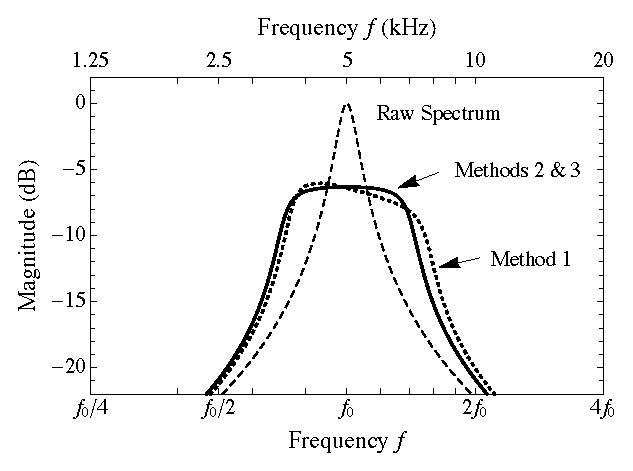
\includegraphics[width=0.6\columnwidth]{a3_smoothing_weights/figures/SmoothedBPFExample.eps}
    \caption[Original and smoothed magnitude responses of a band-pass filter.]{
    Original and 1-octave-smoothed spectra for the magnitude response of an analog band-pass filter.
Method 1 refers to the symmetric weights method; 2 to interpolation to a log-frequency scale; and 3 to log-compensated weights.
The smoothed spectra produced by methods 2 and 3 are nearly identical, so both are represented by the black curve.
The bottom axis shows frequency relative to the center frequency, $f_0$, of the band-pass filter, while the top axis shows frequency in kHz for $f_0 = 5$~kHz.}
    \label{fig:A3_Smoothing_Weights:SmoothedBPFExample}
\end{figure}

The errors in the center of mass are plotted in \figref{fig:A3_Smoothing_Weights:CenterOfMassAnalysis} for each smoothing method and for a range of smoothing bandwidths.
We see from this plot that the center of mass of the smoothed spectrum generated by method 1 increases in frequency as smoothing bandwidth increases.
For small smoothing bandwidths ($\Delta < 1/3$~octave), this error is quite small ($< 1\%$), but becomes large ($\sim 10\%$) for large smoothing bandwidths.

\begin{figure}[t]
    \centering
    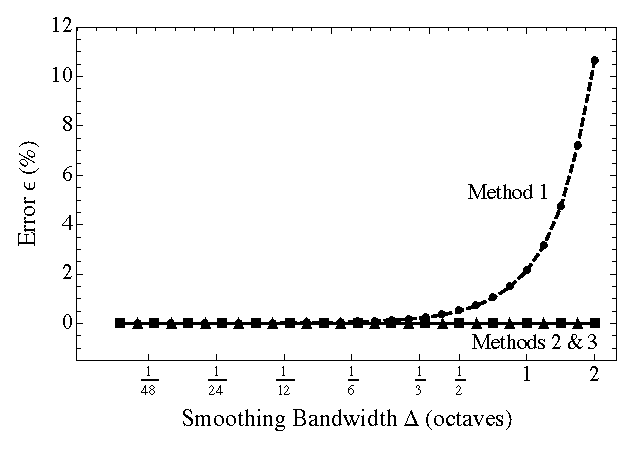
\includegraphics[width=0.6\columnwidth]{a3_smoothing_weights/figures/CenterOfMassAnalysis.eps}
    \caption[Error in the center of mass for different smoothing bandwidths.]{
    Error, $\epsilon$, in the center of mass for different smoothing bandwidths, $\Delta$.
Method 1 refers to the symmetric weights method (denoted by filled circles); 2 to interpolation to a log-frequency scale (triangles); and 3 to log-compensated weights (squares).
Plot markers for methods 2 and 3 are alternated for legibility.}
    \label{fig:A3_Smoothing_Weights:CenterOfMassAnalysis}
\end{figure}

Contrary to the center of mass, the maximum of the smoothed spectrum for method 1 appears shifted to the \textit{left} relative to that of the original spectrum (see \figref{fig:A3_Smoothing_Weights:SmoothedBPFExample}).
To further explore this phenomenon, we apply methods 1 and 3 to smooth a unit impulse located at $f_0$, as shown in \figref{fig:A3_Smoothing_Weights:SmoothingImpulseResponse}.
From this plot we see that the maximum of the smoothed spectrum for method 1 occurs at a significantly lower frequency than $f_0$, although the precise location of the maximum will depend on the raw spectrum (e.g., the width of the raw peak), the smoothing window, and the smoothing bandwidth.

\begin{figure}[t]
    \centering
    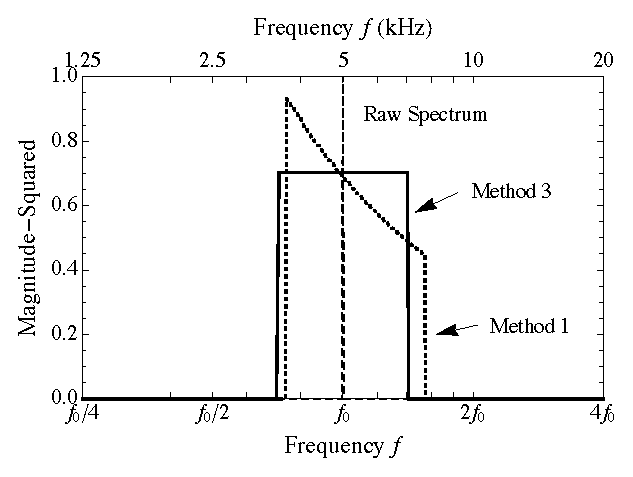
\includegraphics[width=0.6\columnwidth]{a3_smoothing_weights/figures/SmoothingImpulseResponse.eps}
    \caption[Original and smoothed spectra for a unit impulse.]{
    Original and 1-octave-smoothed spectra for a unit impulse located at $f_0$, computed for methods 1 (symmetric weights) and 3 (log-compensated weights).
The smoothed spectra are multiplied by a factor of 100 for legibility.
The bottom axis shows frequency relative to $f_0$, while the top axis shows frequency in kHz for $f_0 = 5$~kHz.}
    \label{fig:A3_Smoothing_Weights:SmoothingImpulseResponse}
\end{figure}

The reason for this shift can be understood in terms of the contribution of the raw spectrum's maximum to each smoothed value.
From \eqnreftwo{eq:A3_Smoothing_Weights:HatzHalfWidth}{eq:A3_Smoothing_Weights:HatzWeights}, as frequency $k$ increases, the width of the smoothing window increases and, due to the normalization of the weights, its amplitude decreases.
Consequently, the contribution of the raw spectrum's maximum to the smoothed value decreases as frequency increases, yielding, in this case, a steadily decreasing smoothed spectrum.

Method 3, on the other hand, creates a uniform spectrum that is symmetric about $f_0$, but has no single maximum.
However, it can be verified that for other smoothing windows (e.g., Hanning), the peak appears at $f_0$.